%% V1.0
%% by Tan Kai Xiong, legendarykx.kaixiong1@gmail.com
%% This is a template for Udacity projects using IEEEtran.cls

%% Be Udacious!

\documentclass[10pt,journal,compsoc]{IEEEtran}

\usepackage[pdftex]{graphicx}
\hyphenation{op-tical net-works semi-conduc-tor}


\begin{document}

\title{Map My World Robot}

\author{Tan Kai Xiong}

\markboth{SLAM project, Robotic Nanodegree, Udacity}%
{}
\IEEEtitleabstractindextext{%

\begin{abstract}
The objective of this project is to perform SLAM (Simultaneous Localization and Mapping) using GraphSLAM to generate a 2D occupancy grids map and 3D mesh point-clouds of two simulated environment in Gazebo. The custom robot model consists of a chassis, two wheel actuators, a RGB-D camera and a 2D LIDAR sensor(Kinect camera and Hokuyo 2D laser scanner). A kitchen environment and a custom office environment will be used in Gazebo. Using the ROS (Robotic Operating System) packages and RTAB-map (Real-Time Appearance Based Mapping) are being used in this project.
\end{abstract}

% Note that keywords are not normally used for peerreview papers.
\begin{IEEEkeywords}
Robot, IEEEtran, Udacity, \LaTeX, SLAM, RTAB-Map.
\end{IEEEkeywords}}


\maketitle
\IEEEdisplaynontitleabstractindextext
\IEEEpeerreviewmaketitle
\section{Introduction}
\label{sec:introduction}

\IEEEPARstart{I}{n} robotics, an autonomous robot must know the environment in order to move safely and accurately to the destination. SLAM estimate the robot's pose and produce a map of the environment. It able to solve the mapping and localization problem at the same time.
    
In this project, two different 3D world scenarios are simulated using Gazebo simulator. The two environments shall be mapped in both 2D and 3D by using Gazebo simulation and ROS frameworks.

\section{Background}
There are two different forms of SLAM. They are online SLAM and full SLAM. The online SLAM solve instantaneous poses independently from previous measurements and controls. The full SLAM need to estimate the entire path instead of an instantaneous pose given all the measurements and controls.
\begin{itemize}
\item Extended Kalman Filter SLAM (EKF)
\item Sparse Extended Information Filter (SEIF)
\item Extended Information Form (EIF)
\item FastSLAM
\item GraphSLAM
\end {itemize}

The two most commonly used methods in robotics are FastSLAM and GraphSLAM. Both algorithms can solve online and full SLAM problems.

\section{FastSLAM}
The FastSLAM algorithm solves the full SLAM problem with known correspondences. It estimates a posterior over the trajectory using a particle filter approach. It uses a low dimensional EKF filter to solve independent features of map which are modeled with local guassian.

\subsection{FastSLAM 1.0}
The FastSLAM 1.0 algorithm is simple and easy to implement, but this algorithm is known to be inefficient since particle filters generate sample inefficiency.

\subsection{FastSLAM 2.0}
The FastSLAM 2.0 algorithm overcomes the inefficiency of FastSLAM 1.0 by imposing a different distribution, which results in a low number of particles. Both FastSLAM 1.0 and 2.0 use a low dimensional EKF filter to estimate the posterior over the map features.

\subsection{Grid-Based FastSLAM}
The Grid-Based FastSLAM is an extension to FastSLAM, which adapts FastSLAM to grid maps. It will update each particle by solving the mapping with known poses problem using the occupancy grid mapping algorithm.

\section{GraphSLAM}
The GraphSLAM using graph-based SLAM approach to constructs a simplified estimation problem by abstracting the raw sensor measurements. The front-end of GraphSLAM looks at how to construct the graph using the odometry and sensory measurements collected by the robot. The back-end is an optimization process that takes all of the constraints and find the system configuration that produces the smallest error.

\subsection{RTAB-Map}
The Real-Time Appearance Based Mapping using the GraphSLAM approach. In RTAB mapping, loop closure is detected using the Bag-Of-Words approach. The Bag-Of-Words is commonly used in vision based mapping. The image features are extracted using the SURF (Speed Up Robust Features). RTAB-Map\cite{rtabmap_ros} uses a memory management technique to limit the number of locations considered as candidates during loop closure detection. This technique is a key feature of RTAB-Map and allows for loop closure to be done in real time.

\section{Robot Model}
A custom differential wheel mobile robot is built in URDF file.  For this type of wheel drive,
it requires two independent motor driven wheels to enable this type of driver to work. It can have either one or two caster wheels to support the robot. It consists of a hokuyo laser scanner, camera and differential wheel sensor.

\begin{figure}[thpb]
      \centering
      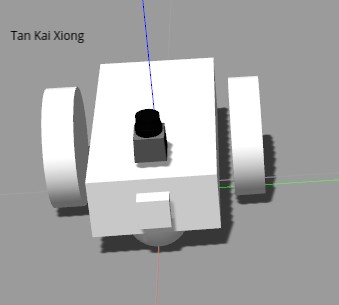
\includegraphics[scale=0.5]{custom_robot.png}
      \caption{Robot Model.}
      \label{fig:robot1}
\end{figure}

\section{Gazebo World}
Gazebo is a 3D robotics simulator. It also features building editor and model editor.

\subsection{Kitchen and Dining}

\begin{figure}[thpb]
      \centering
      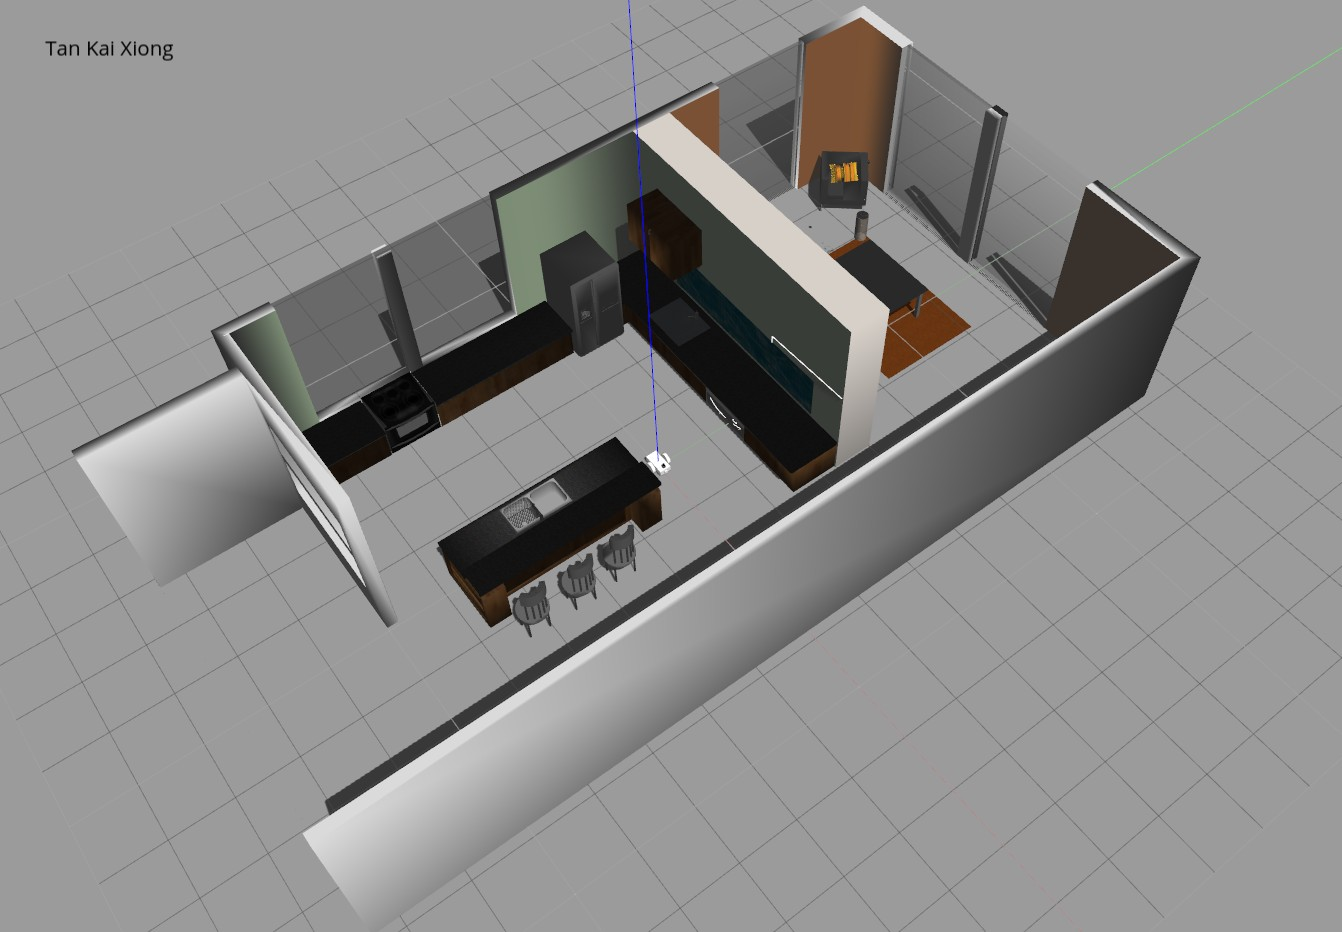
\includegraphics[width=\linewidth]{kitchen_gazebo.png}
      \caption{Kitchen and Dining Gazebo World.}
      \label{fig:robot2}
\end{figure}

\subsection{Custom Office}

\begin{figure}[thpb]
      \centering
      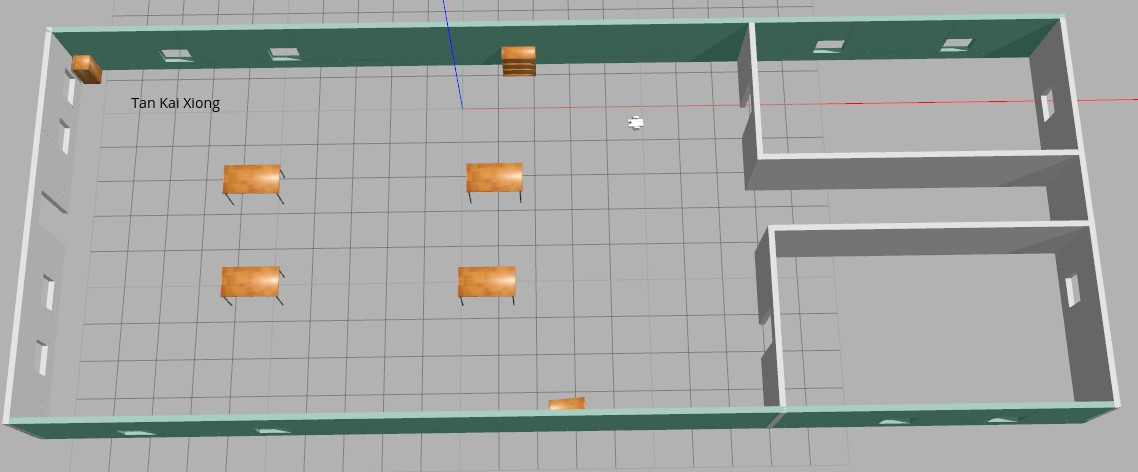
\includegraphics[width=\linewidth]{custom_office_world.png}
      \caption{Custom Office Gazebo World.}
      \label{fig:robot3}
\end{figure}

\section{Result}
Overall, both the 2D and 3D map quality looks good. 

\begin{figure}[thpb]
      \centering
      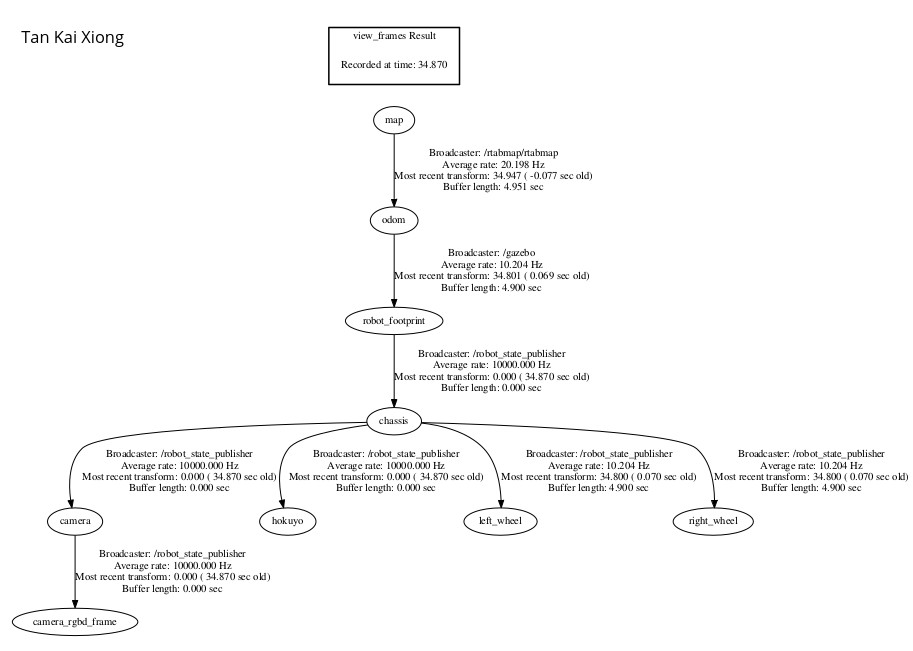
\includegraphics[width=\linewidth]{tf.png}
      \caption{TF tree.}
      \label{fig:robot4}
\end{figure}

\begin{figure}[thpb]
      \centering
      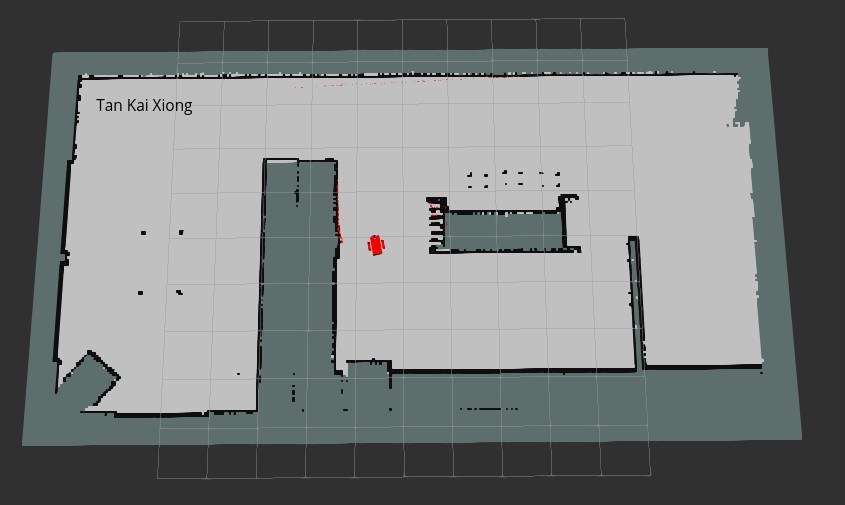
\includegraphics[width=\linewidth]{kitchen_2d_map.png}
      \caption{Kitchen and Dining 2D Grid map.}
      \label{fig:robot5}
\end{figure}

\begin{figure}[thpb]
      \centering
      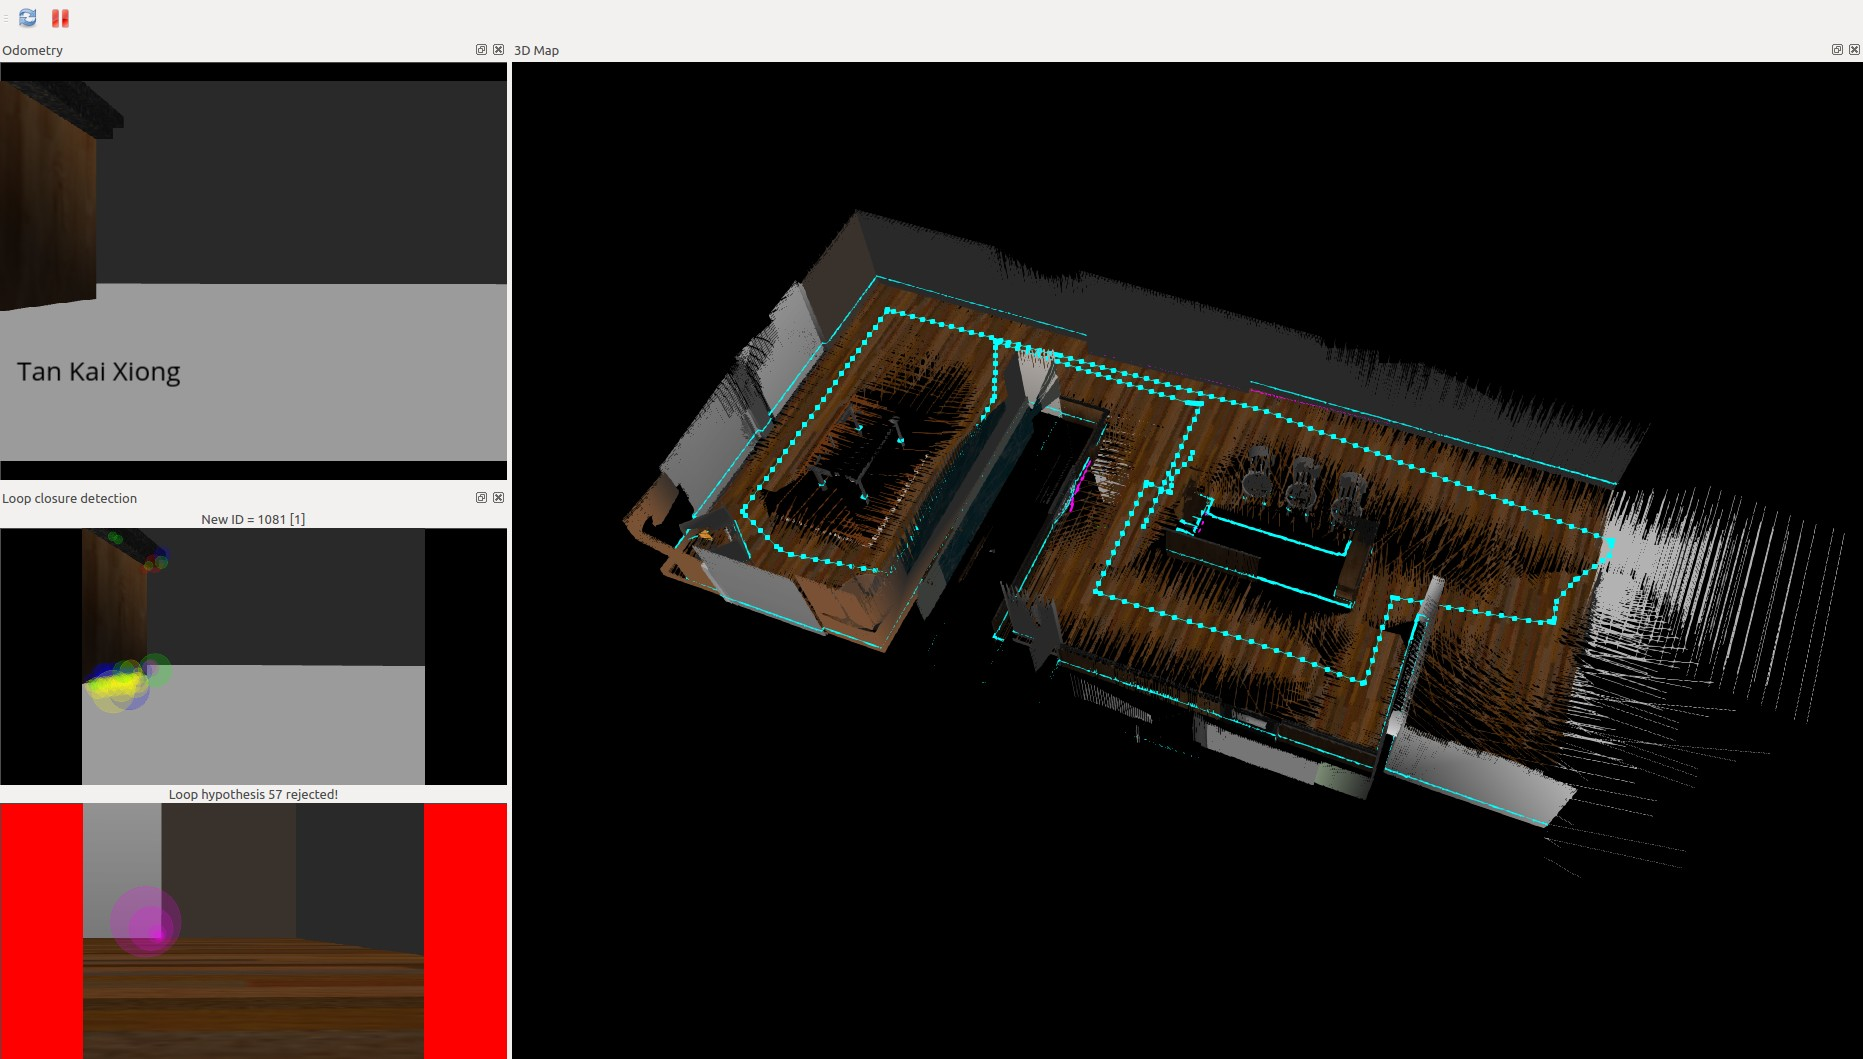
\includegraphics[width=\linewidth]{kitchen_rtabmap.png}
      \caption{Kitchen and Dining RTAB-Map.}
      \label{fig:robot6}
\end{figure}

\begin{figure}[thpb]
      \centering
      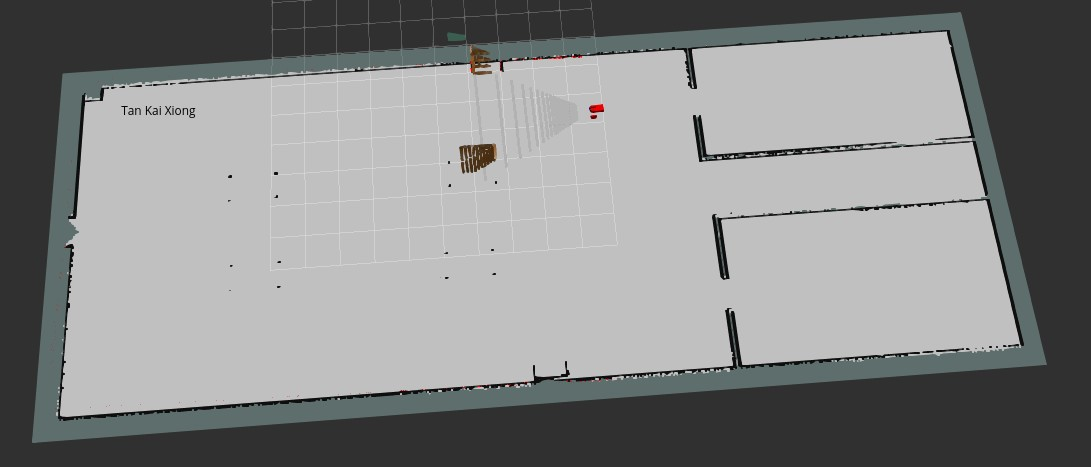
\includegraphics[width=\linewidth]{custom_office_gridmap.png}
      \caption{Custom Office 2D Grid map.}
      \label{fig:robot7}
\end{figure}

\begin{figure}[thpb]
      \centering
      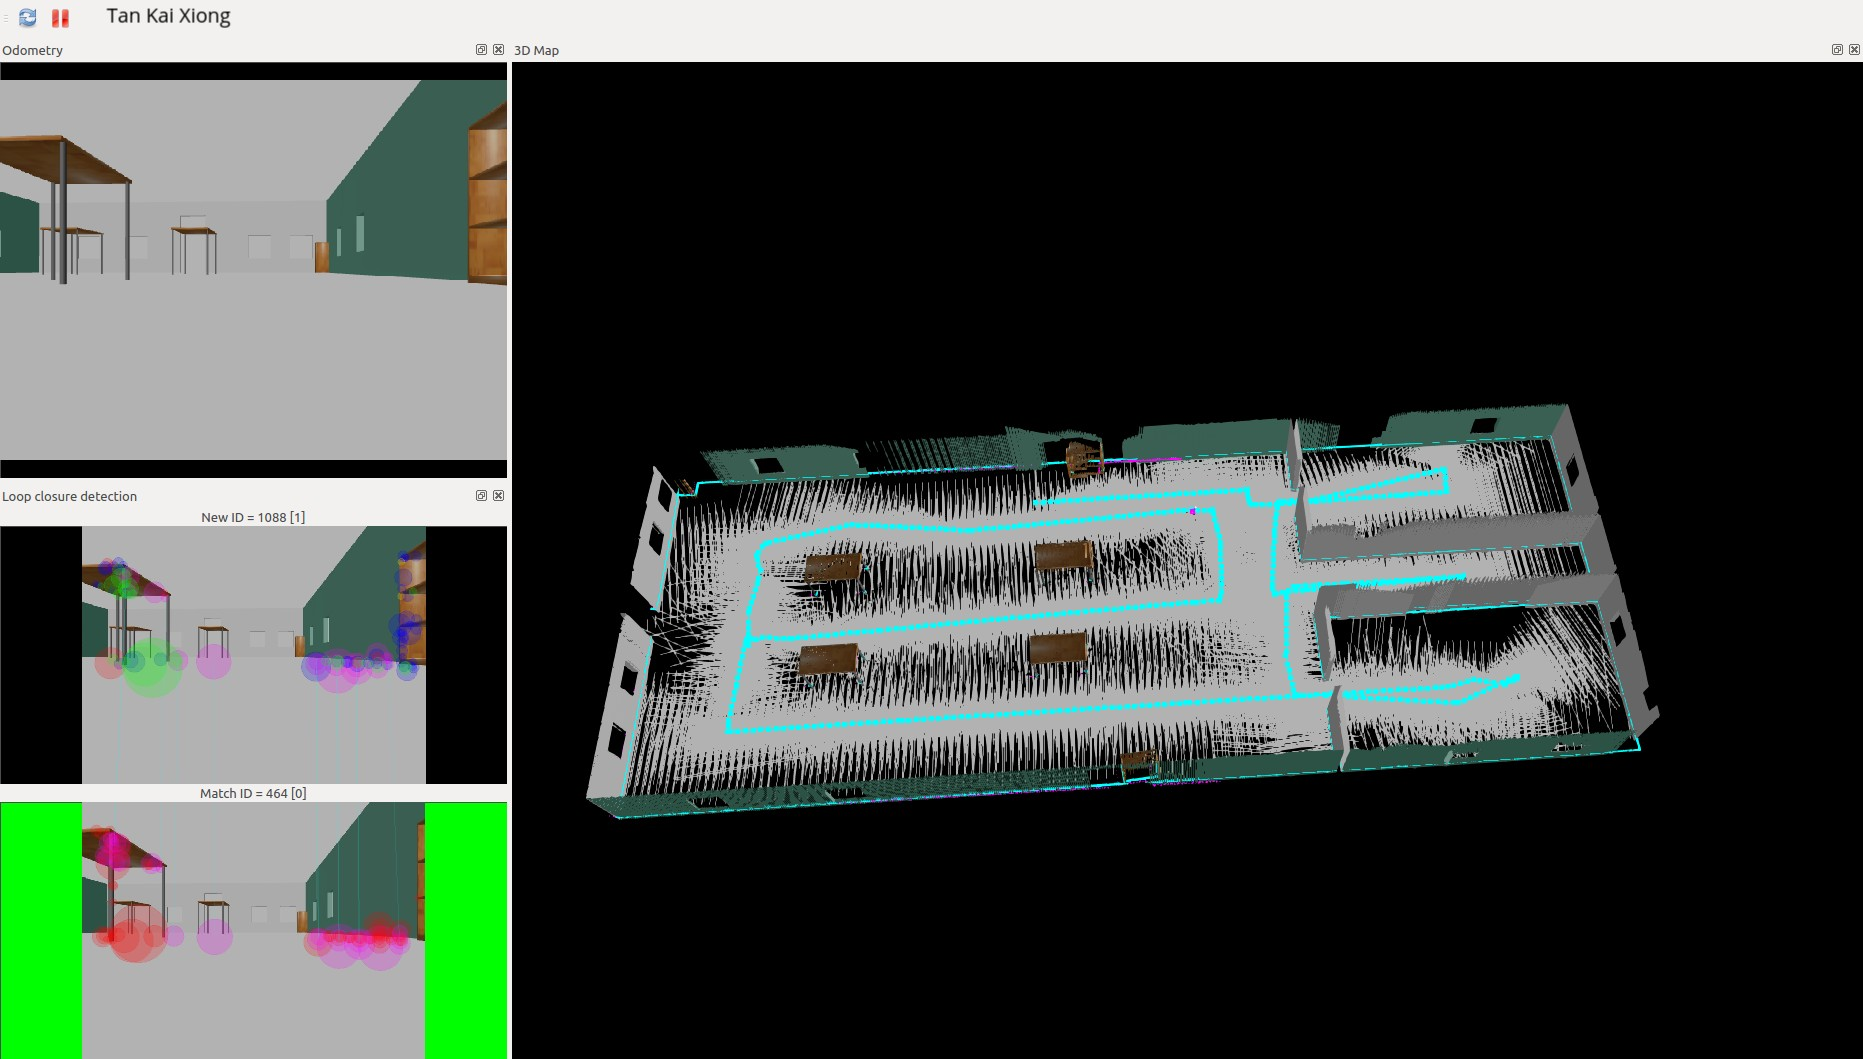
\includegraphics[width=\linewidth]{custom_office_rtabmap.png}
      \caption{Custom Office RTAB-Map.}
      \label{fig:robot8}
\end{figure}

\section{Discussion}
Based on the results, the RTAB-Mapping capable of generating accurate 2D gridmap. There is still some limitation on the RGB-D sensor. The 2D LIDAR able to detect longer distance than RGB-D sensor. The 2D LIDAR can easily map an empty room. In order to generate a full 3D map, the robot have to move nearer to the objects or wall.

\section{Future work}
RTAB-Map is suitable for large scale indoor mapping. The Gazebo editor tools is useful for creating a identical environment to test. 

\bibliography{bib}
\bibliographystyle{ieeetr}

\end{document}